\begin{framed}\noindent
	
	\textbf{Bài 1 - Bài toán đề nghị tháng 8/2018 - Nguyễn Duy Khương}
	
	Cho tam giác $\triangle ABC$ có tiếp điểm đường tròn bàng tiếp góc $\angle A$ với $BC$ là $E$. Gọi $K$ là hình chiếu của $E$ lên đường trung bình ứng với đỉnh $A$ của tam giác $\triangle ABC$. Chứng minh $(K, KE)$ tiếp xúc với $(O)$.

	
\end{framed}

\textbf{Lời giải 1 - Nguyễn Duy Khương.}

Đổi mô hình coi vai trò mới của $(O)$ là đường tròn $(BOC)$ bài toán trở thành bài toán sau: 

\textbf{Bài toán mới - Trần Quang Hùng (AoPS).} Cho tam giác $ABC$ nội tiếp $(O)$. $AO\cap BC,(BOC)=M,N$ và $P$ là trung điểm $MN$. Hạ $PK\perp AH(K\in AH)$ với $H$ là chân đường cao hạ từ $A$ xuống $BC$. Chứng minh rằng: $(H,HK)$ tiếp xúc $(BOC)$.

\begin{center}
	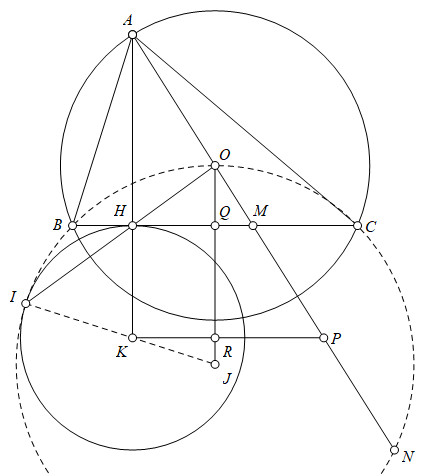
\includegraphics[scale=0.6]{T082018/T82018_KhuongNguyen_SOL1}
	
\end{center}

\textbf{Chứng minh bài toán mới.}

Gọi $Q$ là trung điểm $BC$. Gọi $OH\cap (BOC)=I,O$ ta có: $OH.OI=OB^2$ suy ra: $OI=\dfrac{R^2}{OH}$ suy ra: $\dfrac{IH}{OI}=1-\dfrac{OH^2}{R^2}=1-\dfrac{OQ^2+\dfrac{ST^2}{4}}{R^2}
=1-(cos{A})^2-(cos{ACS})^2=(sin{A})^2-(sin(B-C))^2=(sinA-sin(B-C))(sinA+sin{(B-C)})=sin2B.sin2C$.

Gọi $J$ là tâm của $(BOC)$, ta có $\dfrac{OB}{2OJ}=cosA$ suy ra  $OJ=\dfrac{R^2}{2OQ}$. 

$KP\cap OQ = R$, ta có $HKRQ$ là hình chữ nhật do đó $HK=QR$.

Ta có: $\dfrac{QR}{OQ}=\dfrac{MN}{2OM}$ suy ra: $QR=\dfrac{MN.OQ}{2OM}$ suy ra: $\dfrac{OJ}{HK}=\dfrac{R^2.OM}{OQ^2.MN}$. Theo bổ đề cát tuyến ta có: $\dfrac{OM}{MN}=\dfrac{OB}{BN}.\dfrac{OC}{CN}=
\dfrac{cosA.cosA}{sin2C.sin2B}$ mà $\dfrac{R^2}{OQ^2}=\dfrac{1}{(cos{A})^2}$. Vậy ta có: $\dfrac{HK}{OJ}=sin2B.sin2C$.  

Tóm lại ta có: $\dfrac{HK}{OJ}=\dfrac{IH}{OI}$ do đó: $I,K,J$ thẳng hàng dẫn đến: $(K;KH)$ tiếp xúc $(BOC)$.

Như vậy tức là bài toán gốc cũng đúng. $\qquad \blacksquare$

Ngay sau những ngày đầu tiên của chuyên mục, \textbf{bài toán 1} đúng như vị trí của nó đã được các bạn đón nhận nhiều nhất với rất nhiều lời giải khác hẳn lời giải gốc. Tư duy đổi mô hình cũng được bạn \textbf{Zeref} trên VMF tận dụng rất điêu luyện từ đó có 1 lời giải rất hay.

\textbf{Lời giải 2 - Zeref}.

Xét bài toán sau: Cho tam giác $\triangle ABC$ có $AD, BE, CF$ là các đường cao. Gọi $G$ là hình chiếu vuông góc của $A$ lên $EF$ và $L$ là hình chiếu của $D$ lên $AG$. Chứng minh $(GL)$ tiếp xúc với $(DEF)$.

Vai trò của tam giác $\triangle DEF$ và $(GL)$ trong bài toán này tương tự vai trò của tam giác $\triangle ABC$ và $(K, KE)$ ở bài toán gốc.

\begin{center}
	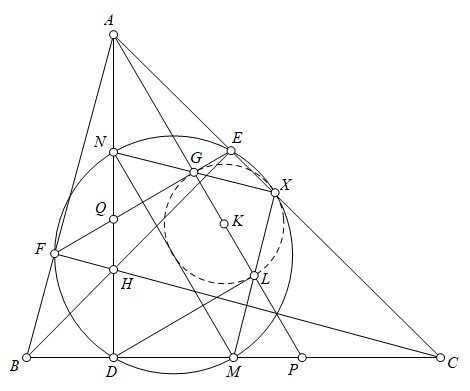
\includegraphics[scale=0.6]{T082018/T82018_KhuongNguyen_SOL2}
	
\end{center}

Gọi $H$ là trực tâm, $M,N$ là trung điểm $BC,AH$. $AG \cap BC=P$ và $AH \cap EF=Q$. Gọi $K$ là trung điểm $GL$. Ta sẽ chứng minh $NG \perp ML$.

Do $(AH,QD)=-1$ nên $NA^2=NQ.ND \Rightarrow  \dfrac{NA}{NQ}=\dfrac{ND}{NA}=\dfrac{MD}{MP}$

Mà $\triangle GAQ \sim \triangle LDP$ (chú ý các tam giác vuông). Do đó $\triangle AGN \sim \triangle DLM$.

Ta có: $\widehat{GNM}+\widehat{LMN}=\widehat{AGN}+\widehat{LMN}=\widehat{DLM}+\widehat{LMN}=90^o$

Do đó $NG \perp ML$. Gọi $X=NG \cap ML$. $\widehat{NXD}=90^o$ nên $X \in (DEF)$. Và $GL \parallel MN \Rightarrow X \in (K;KG)$ 

Vậy $X \in (K;KG),(DEF)$ và $GL \parallel MN$ nên $(K;KG)$ tiếp xúc $(DEF)$. $\qquad \blacksquare$

Sử dụng mô hình gốc để chứng minh là một hướng đi khó nhưng đã có hai lời giải hay của các bạn \textbf{Nguyễn Duy Khang-TPHCM} và \textbf{Nguyễn Hà An-12 Toán THPT chuyên ĐHSP} cho hướng đi này. Ngoài ra còn có bạn \textbf{Trần Quốc Thịnh} có lời giải giống bạn Hà An (cách xử lí có dài hơn). Cách xử lí tiếp điểm của bạn An và Thịnh rất chuẩn xác. Tư duy điểm trùng và tỉ số của Khang cũng rất đặc sắc. Xin giới thiệu hai lời giải của bạn Khang và An.

\textbf{Lời giải 3 - Nguyễn Hà An.}

\begin{center}
	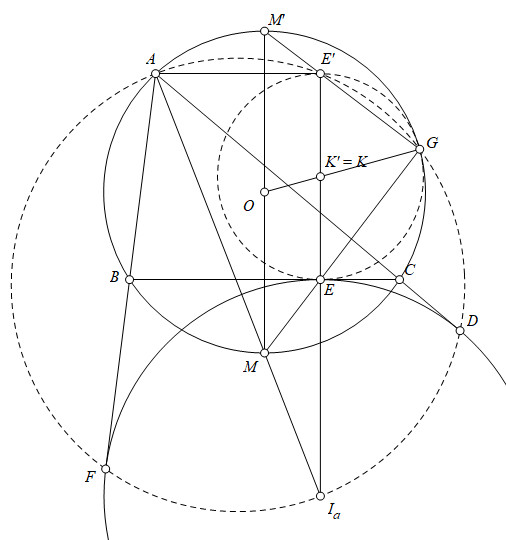
\includegraphics[scale=0.6]{T082018/T82018_KhuongNguyen_SOL3}
	
\end{center}

Gọi $I_a$ là tâm bàng tiếp, $D,F$ là tiếp điểm của $(I_a)$ với $CA, AB$. Gọi $M,M'$ là trung điểm cung nhỏ, cung lớn $\arc {BC}$, $(AI_a)$ cắt $(O)$ tại $G \neq A$.

Dễ thấy $\triangle GBF \sim \triangle GCD => \dfrac{GB}{GC}=\dfrac{BF}{CD}=\dfrac{BE}{CE} => GE$ là phân giác $BGC$ hay $G,E,M$ thẳng hàng.

Gọi $K'=OG \cap IaE$ thì do $KE \parallel OM$ và $\triangle OGM$ cân tại $O => K'E=K'G => (K',KE)$ tiếp xúc $(O)$ tại $G$.

Lấy $E'$ đối xứng $E$ qua $K'$ thì $\angle EGE'=90^o=\angle MGM'$ mà $M,E,G$ thẳng hàng nên $G,E',M'$ thẳng hàng.

Vì vậy $\angle AGE'=\angle AGM'=\angle AMM'=\angle AIaE'$ => $A,E',G,Ia$ nội tiếp hay $AE'\parallel BC$. Từ đó có $K'$ thuộc đường trung bình đỉnh $A$. Vậy $K' \equiv K $ hay $(K,KE)$ tiếp xúc $(O)$. $\qquad \blacksquare$

\textbf{Lời giải 4 - Nguyễn Duy Khang.}

\begin{center}
	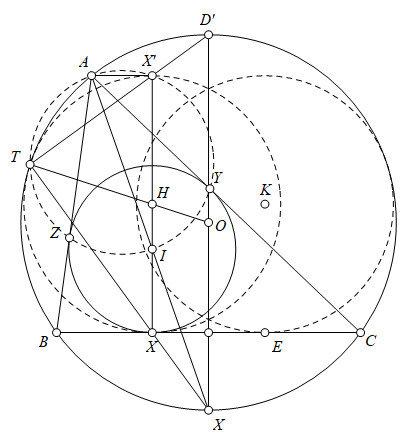
\includegraphics[scale=0.6]{T082018/T82018_KhuongNguyen_SOL4}
	
\end{center}

Gọi $(I)$ là đường tròn nội tiếp tam giác $\triangle ABC$. $(I)$ lần lượt tiếp xúc với $BC, CA, AB$ tại $X, Y, Z$. Gọi $T$ là giao điểm thứ hai của $(AI)$ và $(O)$. Ta có kết quả $TX$ đi qua $D$ là điểm chính giữa cung nhỏ $\arc {BC}$ của $(O)$.

Gọi $H = IX \cap OT$, nhận thấy $(H, HX)$ tiếp xúc với $(O)$ tại $T$, ta sẽ chứng minh $H, K$ đối xứng với nhau qua trung trực của $BC$.

Gọi $D'$ đối xứng với $D$ qua $O$, $X'$ đối xứng với $X$ qua $H$, theo bổ đề hình thang thì $T, X', D'$ thẳng hàng.

Do $DD'$ là đường kính của $(O)$ nên $\angle ATX' = \angle ADD' = \angle DIX = \angle AIX'$, suy ra $X'$ nằm trên $(AI)$. Do $AX' \bot XX'$ và $AX' \parallel BC$ kết hợp với $H$ là trung điểm của $XX'$ suy ra $H$ nằm trên đường trung bình ứng với đỉnh $A$ của tam giác $\triangle ABC$.

$X, E$ đối xứng với nhau qua $DD'$ suy ra $H, K$ đối xứng với nhau qua $DD'$, do đó $(H, HX)$ và $(K, KE)$ đối xứng với nhau qua $DD'$. Vậy $(K, KE)$ tiếp xúc với $(O)$. $\qquad \blacksquare$